% !TeX spellcheck = ru_RU
% !TEX root = vkr.tex

\section{Эксперимент}

Целями следующих экспериментов является выявление возможности зависимости пропускной способности рантайма от взаимодействия воркеров с глобальной очередью. Это взаимодействие будет оцениваться c помощью выделенных метрик.

Каждая задача спавнер помещается в отдельный блокирующий поток путем вызова \verb|spawn_blocking| и спецификации рантайму \verb|max_blocking_threads| равному количеству спавнеров. Каждая задача продуцирует одинаковое количество пустых листовых задач. Дабы избежать оптимизации редуцирующей тело задачи в нее помещена непрозрачная для компилятора функция-пустышка \verb|std::hint:black_box|.

\subsection{Условия эксперимента}

Исследования проводились на системе YADRO VEGMAN Rx20 G2\footnote{\href{https://yadro.com/ru/vegman/rx20g2/specs}{Описание} сисемы YADRO VEGMAN Rx20 G2}. Бенчмарк был запущен с значением \verb|nice| равным минус двадцати.

Машина для измерение производительности была любезно предоставлена командой \verb|TATLIN.BACKUP| и находилась удаленно, в связи с чем на ней было невозможно отключение сети.

\subsubsection{Метрики}

Метрики были получены путем произведения тридцати итераций прогрева с последующими ста итерациями исполнения на отдельном инстансе рантайма, после чего метрики подвергались экстракции из последнего.

\subsection{Ход исследования}

\begin{figure}[H]
    \begin{center}
        \makebox[\textwidth]{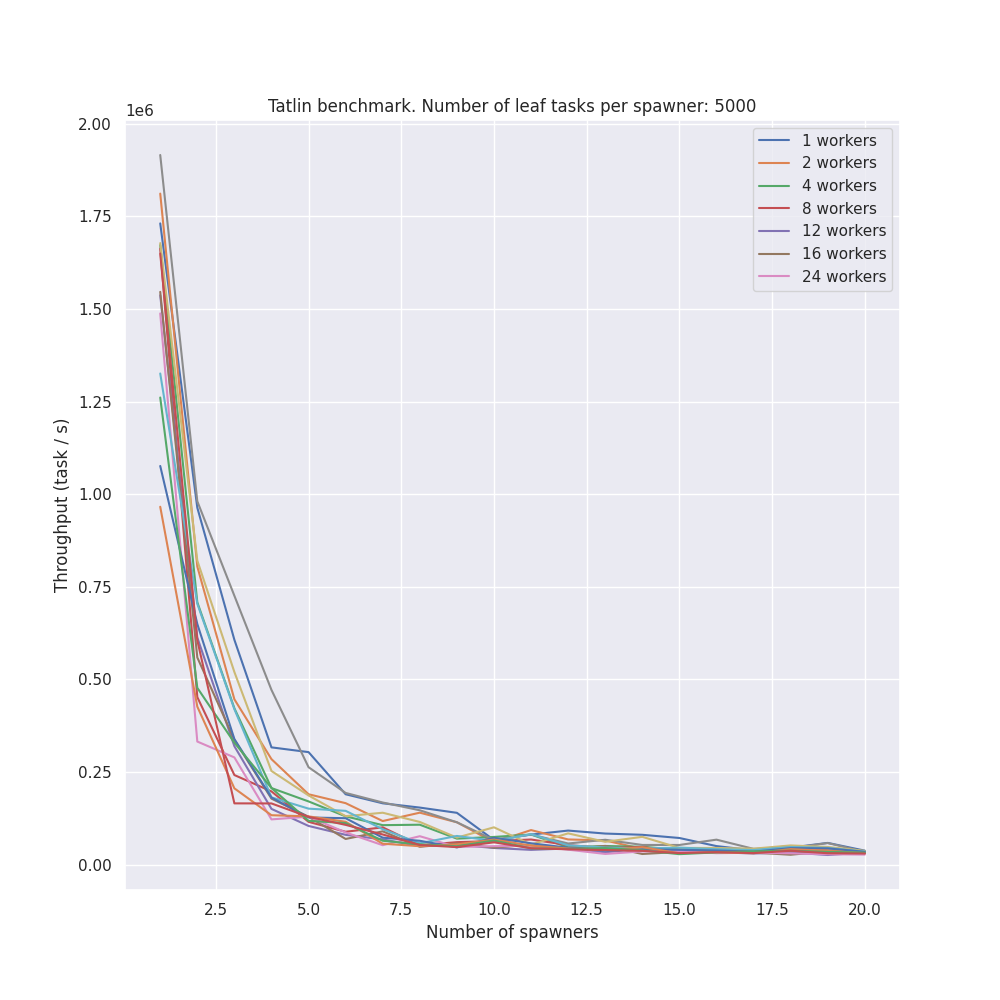
\includegraphics[scale=0.70]{pictures/blocking/tatlin_blocking.png}}
    \end{center}

    \caption{Пропускная способность в зависимости от количества спавнеров}
    \label{fig:tatlin:line:nspawn:5000}
\end{figure}

Как видно из графика \ref{fig:tatlin:line:nspawn:5000}:

\begin{itemize}
    \item Пропускная способность рантайма падает с увеличением количества спавнеров независимо от количества воркеров
    \item При увеличении количества воркеров падение становится более стабильным, что отражено на рисунке \ref{fig:tatlin:line:nspawn:5000:from:8}
    \item Исключением являются результаты одного воркера, где для малого количества спавнеров заметен рост
\end{itemize}

\begin{figure}[H]
    \begin{center}
        \makebox[\textwidth]{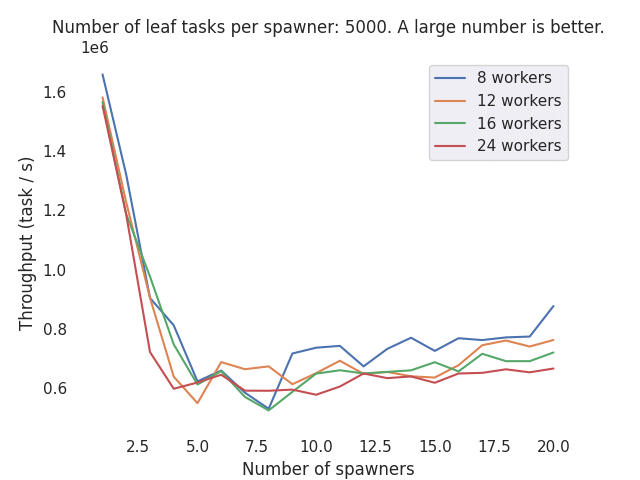
\includegraphics[scale=0.70]{pictures/blocking/tatlin_blocking_from_8.png}}
    \end{center}

    \caption{Пропускная способность в зависимости от количества спавнеров}
    \label{fig:tatlin:line:nspawn:5000:from:8}
\end{figure}

Источником задач для воркеров в данном случае является глобальная очередь. Воркеры могут делиться задачами с помощью механизма стилинга, однако получать новые задачи они способны исключительно благодаря взаимодействию с глобальной очередью, которая требует эксклюзивного владения для добавления и изъятия задач.

Зависимость операций стилинга от количества спавнеров приведена на графике \ref{fig:tatlin:metrics:steal_ops}:

\begin{itemize}
    \item В случае одного воркера, количество похищений равно нулю --- воркеров всего один
    \item В других случаях количество похищений растет, затем падает. Вероятно, при достаточном насыщении глобальной очереди воркеры более не прибегают к попытке похищения и довольствуются задачами из глобальной очереди
\end{itemize}

\begin{figure}[H]
    \begin{center}
        \makebox[\textwidth]{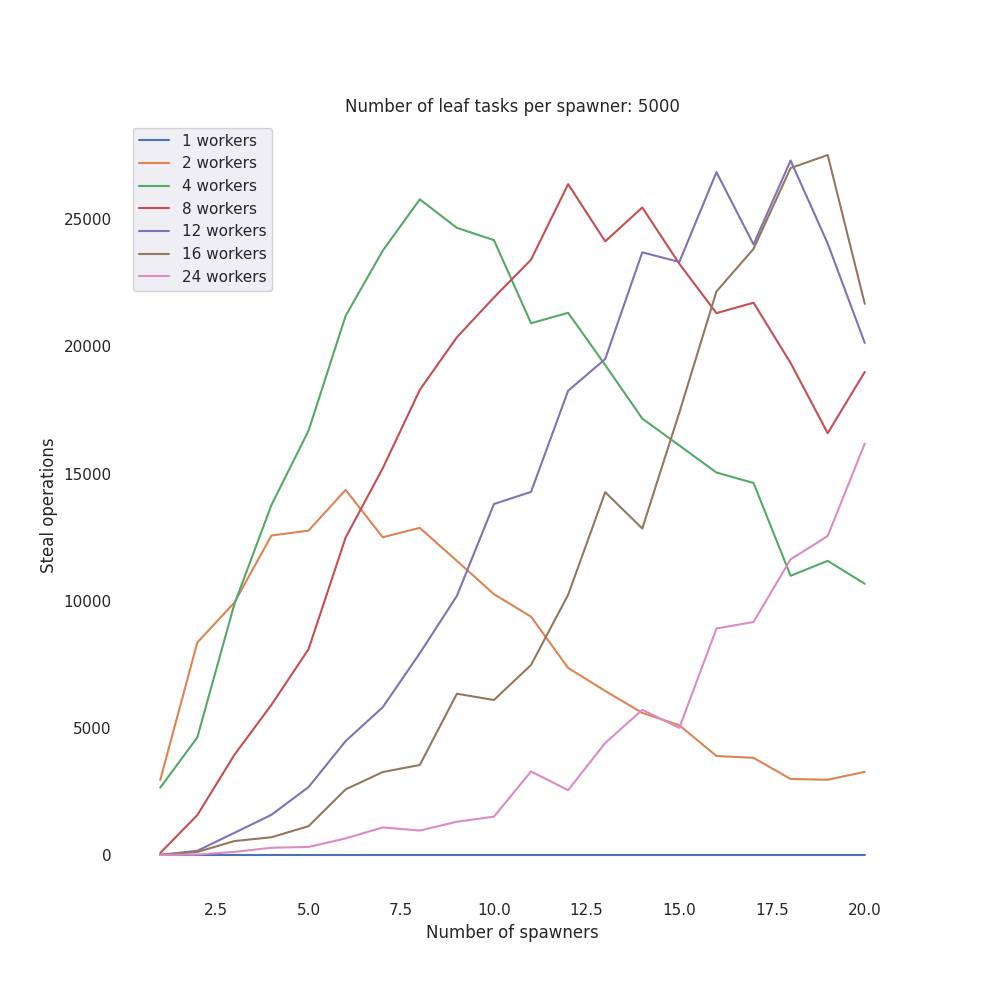
\includegraphics[scale=0.40]{pictures/steal_worker.png}}
    \end{center}

    \caption{Количество похищений относительно количества спавнеров}
    \label{fig:tatlin:metrics:steal_ops}
\end{figure}

Стилинг скорее всего несет накладные расходы, но падение пропускной способность с увеличением количества спавнеров наблюдается в случае одного воркера, где стилинг отсутствует. Стоит заметить: с уменьшением количества операций стилинга рост пропускной способности не наблюдается.

\subsection{Использование нескольких рантаймов}

\begin{figure}[H]
    \begin{center}
        \makebox[\textwidth]{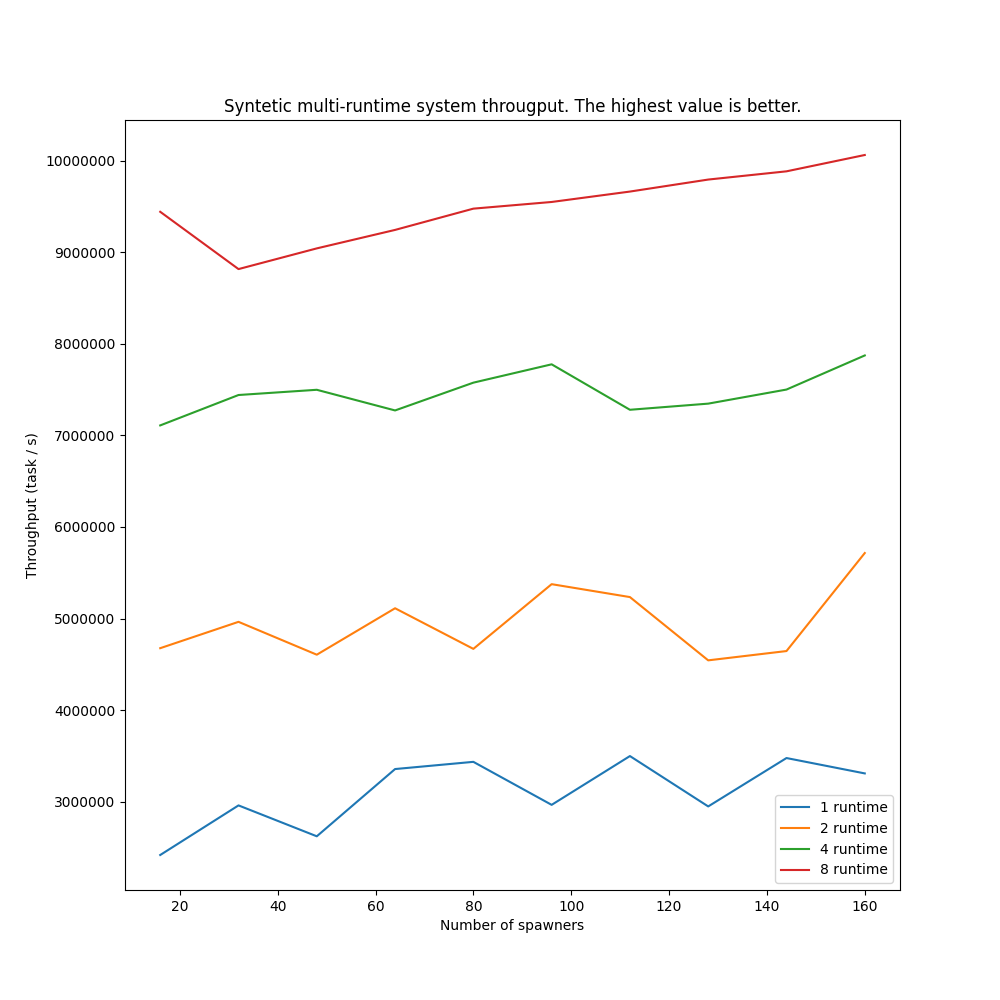
\includegraphics[scale=0.40]{pictures/multi_rt_eval.png}}
    \end{center}

    \caption{Производительность системы при использовании нескольких рантаймов}
    \label{fig:tatlin:multi_rt:eval}
\end{figure}

\subsection{Вывод}

Глобальная очередь может накладывать ограничение на производительность всего рантайма в следствие борьбы за добавление новых задач из блокирующих потоков и попыток изъятия потоками воркеров.
